\documentclass[a4paper,12pt]{article}
\usepackage{amsfonts}
\usepackage{amssymb}
\usepackage{latexsym}
\usepackage{amsmath}
\usepackage{amsthm}
\usepackage{graphicx}
\usepackage{indentfirst}
\usepackage[polish]{babel}
\usepackage[T1]{fontenc}
\usepackage[utf8]{inputenc}
\usepackage{wrapfig}
%\usepackage[cp1250]{utf8}
\usepackage{setspace}
\usepackage{array}
\usepackage{multirow}
\usepackage{geometry}
\geometry{hdivide={2cm,*,2cm}}
\geometry{vdivide={2cm,*,2cm}}
\usepackage{titlesec}
%\captionsetup[table]{position=bottom}
\titlespacing{\section}{0ex}{1ex}{1ex} % zmniejszenie odstêpów przed i po tytule rozdzia³u...
\titleformat*{\section}{\sf\large\bfseries} % i zmiana kroju czcionki
\titlespacing{\subsection}{0ex}{0.75ex}{0.75ex} % % j/w dla tytu³ów podrozdzia³ów
\titleformat*{\subsection}{\sf\bfseries}

% Zmniejszenie odstêpów przed i za wzorami wystawionymi
\AtBeginDocument{
\addtolength{\abovedisplayskip}{-1ex}
\addtolength{\abovedisplayshortskip}{-1ex}
\addtolength{\belowdisplayskip}{-1ex}
\addtolength{\belowdisplayshortskip}{-1ex}
}
% Kilka przydatnych definicji
\newcolumntype{C}[1]{>{\centering\arraybackslash}m{#1}}
\newcommand{\razy}{\hspace{-0.5ex}\times\hspace{-0.5ex}} % mo¿e siê przydaæ

\begin{document}
\def\tablename{Tabela} % bez tej linii nazw¹ tabeli by³aby "Tablica"
\noindent
\textbf{Sebastian Prokop, 320728, grupa 4, projekt 1, zadanie 52}

%%% Nie do końca rozumiem wszystko co się dzieje powyżej. Poniżej jest część, którą ja zrobiłem 

\section*{Wstęp}
Formuła całkowa jaką jest metoda trójkątów rzędu czwartego to sposób na wyznaczanie przybliżonej wartości całki podwójnej na określonym obszarze skończonym. Jednym z rodzajów funkcji dwóch zmiennych są wielomiany stopnia $n$ - w sekcji \emph{Testy poprawności} scharakteryzowane formalnie. Dla tych rzędu mniejszego niż 4 metoda jest dokładna, nastomiast dla rzędów większych niż 3, znana jest teoretyczna maksymalna wartość błędu.

Raport ten potwierdza teoretyczne założenia dotyczące rzędu i dokładności badanej metody i omawia własności numeryczne jej implementacji. Jak się okazuje, choć metoda jest dokładna dla odpowiednich rzędów, w implementacji mogą pojawiać się drobne błędy w zależności od doboru parametru n. 
\section*{Opis formuły całkowej $S_{SWK} (f)$}
Opisywana metoda opiera się na podziale obszaru na trójkąty i obliczaniu wartości funkcji w siedmiu charakterystycznych miejscach każdego trójkąta z odpowiednimi wagami. Są to wierzchołki, środki boków i środek trójkąta, oznaczane kolejno: $p_0, p_1, p_2, p_{01}, p_{02}, p_{12}, p_{012}$, gdzie:
\[ p_{01} = \frac{1}{2} (p_0 + p_1), \;  p_{02} = \frac{1}{2} (p_0 + p_2), \; p_{12} = \frac{1}{2} (p_1 + p_2), \; p_{012} = \frac{1}{3} (p_0 + p_1 + p_2),\]
Wartość całki $S$ na trójkącie jest przybliżana za pomocą wzoru:
\[  S = \frac{P}{60} (27f(p_{012}+3(f(p_0)+f(p_1)+f(p_2))+8(f(p_{01}) + f(p_{02}) + f(p_{12})), \]
gdzie P jest polem trójkąta.
W związku z tym wartosć całki przy podziale obszaru na t trójkątów przystających jest przybliżana sumą po wszystkich trójkątach:
\[ \sum_{i=1}^{t} S_i. \]

\section*{Opis funkcji}

\begin{wrapfigure}{R}{0.25\textwidth} %this figure will be at the right
    \centering
    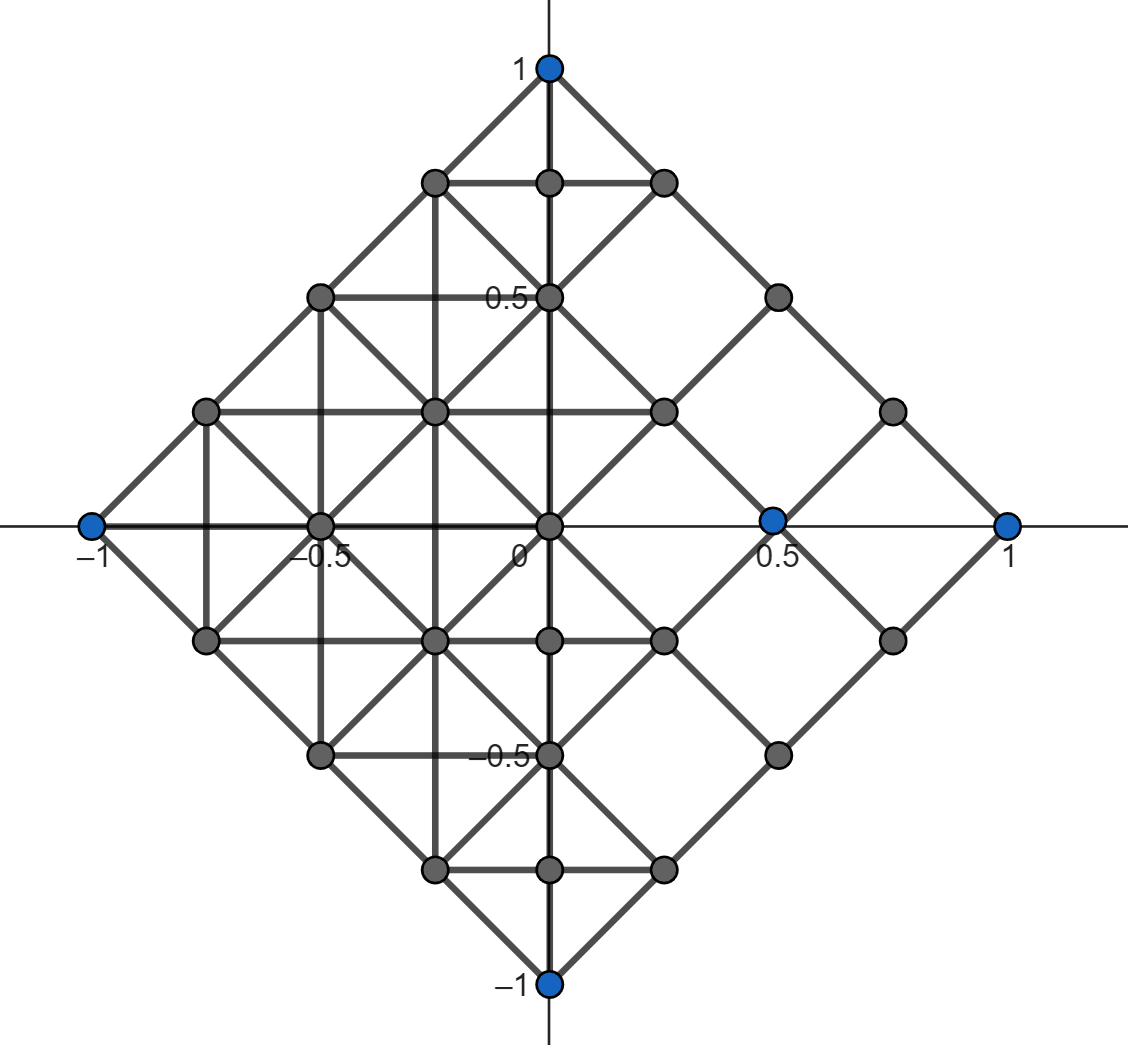
\includegraphics[width=0.25\textwidth]{rys1.png}
     \footnotesize \caption{ Obszar w trakcie podziału. Każdy z $n^2$ kwadratów $(n=4)$ jest dzielony na 4 trójkąty}
\end{wrapfigure}
Żeby skorzystać z omawianej metody trójkątów, podzielimy zadany obszar na trójkąty przystające. Obszar, o którym mowa jest określony następująco:
\[ D = \{ ( x,y) \in R^2: |x| + |y| \leq 1 \}. \]
Jest to romb o środku w punkcie $(0,0)$ i boku długości $\sqrt{2}$. Jest on dzielony na $4n^2$ trójkątów przystających, poprzez podział boków na $n$ odcinków, nasępnie podział rombu na $n^2$ kwadratów i ostatecznie podział każdego małego kwadratu na 4 trójkąty poprzez poprowadzenie przekątnych. Moment w trakcie podziału przedstawia rysunek po prawej.



\section*{Testy poprawności i precyzji}
Żeby sprawdzić, czy formuła jest faktycznie czwartego rzędu, należy sprawdzić wielomiany stanowiące bazę przestrzeni wielomianów stopnia mniejszego niż 4, gdzie przestrzeń wielomianów stopnia n jest określana jako:
\[ W_n = \{ p: p(x,y) = \sum_{0 \leq q+r \leq n} a_{qr}x^qy^r, a_{qr} \in R \} \]
Wszystkie wielomiany stopnia mniejszego niż 4 będą kombinacją liniową wektorów z bazy, co w połączeniu z własnościami całki oznaza, że wystarczy policzyć całki z bazy.

Badany obszar jest symetryczny względem obu osi, przez co całki z funkcji nieparzystych będą równe zero. Niezerowy wynik z wzoru 
\[ \iint_D f(x,y) \,dx\,dy \]
otrzymamy dla $1$, $x^2$, $y^2$:
\[ \iint_D 1 \,dx\,dy = 2 \;\;\; , \;\;   \iint_D x^2 \,dx\,dy =  \iint_D y^2 \,dx\,dy = \frac{1}{3} \]
Wyniki działania funkcji dla $n=1$ faktycznie dają dokładnie takie wartości, natomiast dla pozostałych wektorów z bazy (wszystkie wymienione w teście pierwszym) zwraca zera. 

Kolejne testy dotyczą błędu przy wielomianach stopni wyższych niż trzeci. Jego wartość można ograniczyć zgodnie ze wzorem:
\[ |I(f) - S(f) | = \mathcal{O}(n^{-4}), \]
gdzie $I(f)$ to dokładna wartość a $S(f)$ przybliżona. Wzór tyczy się podziału trójkątnego obszaru na $n^2$ trójkątów. W przypadku omawianego zadania są 4 obszary trójkąte i podział na $4n^2$ trójkątów, dlatego nadal możemy posługiwać się tym wzorem. Tabela poniżej przedstawia wyniki obliczeń wykonane na kilku przykładowych funkcjach na potrzeby sprawdzenia jego poprawności.

\begin{table}[h]
\begin{center}
\begin{tabular}{lllll}
\textbf{Wzór funkcji} & \textbf{Poprawny} & \textbf{Programu} & \textbf{Błąd} & \textbf{Stosunek} \\
\hline
$x^4$ & $\frac{2}{15}$ & 0.13333 & 1.1111e-10 & 0.011111 \\
$x^2 \razy y^2 $& $\frac{1}{45}$ & 0.022222 & 5.5556e-11 & 0.0055556 \\
$x^5$ & 0 & 2.0956e-16 & 2.0956e-16 & 2.0956e-08 \\
$x^4 + y^4 + 2xy + 1 $& $\frac{34}{15}$ & 2.2667 & 2.2222e-10 & 0.022222 
\end{tabular}
\footnotesize \caption{\label{1}Porównanie błędu z maksymalnym teoretycznym dla przykładowych funkcji}
\end{center}
\end{table}
\vspace{-6mm}%Put here to reduce too much white space after your table
Kolumna \emph{Stosunek} to iloraz błędu i maksymalnego teoretycznego błędu. Wszystkie wartości zostały wyliczone dla $n=100$. Jeżeli stosunek jest mniejszy niż 1 znaczy to, że błąd był mniejszy niż maksymalny teoretyczny. Do sprawdzenia jak wygląda podobna tabela dla różnych wartości n służy \emph{test3}. Niezależnie od funkcji i parametru, stosunek zawsze wychodzi mniejszy niż 1. 

\section*{Testy numeryczne}
Pierwsza kwestia, którą warto omwówić w kontekście poprawności numerycznej jest czas działania i zależność czasu liczenia od parametru n i funkcji f. Poniższa tabela przedstawia przykładowe funkcje i czasy obliczeń dla rónych n (więcej w \emph{test5}). Jak widać największy wpływ na czas obliczeń ma wzór funkcji - czy jest skomplikowany, czy nie wymaga wielu obliczeń.

\begin{table}[h]
\begin{center}
\begin{tabular}{lllll}
\textbf{Wzór funkcji} & \textbf{n = 5} & \textbf{n = 50} & \textbf{n = 500} & \textbf{n = 5000} \\
\hline
$1$                    &  8.8360e-04 & 4.4750e-04 & 0.0062 & 0.7753\\
$x \razy y $           &  6.5170e-04 & 4.4800e-04 & 0.0074 & 0.0074\\
$x^4 + y^4 + 2xy + 1 $ &  8.7200e-04 & 114.0e-04  & 0.3780 & 35.2911\\
\end{tabular}
\footnotesize \caption{\label{2}Porównanie czasu obliczeń dla różnych funkcji i wartości n.}
\end{center}
\end{table}
\vspace{-6mm}%Put here to reduce too much white space after your table
Druga kwestia na którą warto zwrócić uwagę, to błędy precyzji obliczeń. Gdyby dla policzenia wielomianu stopnia drugiego użyć $n$ takiego, że któreś punkty będą miały współrzędne, których zapis ma nieskończone rozwinięcie, to liczona będzie wartość bardzo bliska ale nie dokładnie w poprawnym puknkcie. Tak więc dla $f(x,y) = xy$ i $n=10$ wynik działania funkcji zamiast 0 wynosi okolo $10^{-17}$.

\section*{Funkcje inne niż wielomianowe}
Do badania dokładności przybliżania funkcji innych niż wielomianowe służy \emph{test5}. Metoda trójkątów czwartego rzędu okazuje się być dobrą metodą przybliżania całek podwójnych.

\end{document}